\documentclass{beamer}

\mode<presentation> {
%	\usetheme{Berlin}
	\usecolortheme{default}
	\usefonttheme{serif}
\setbeamertemplate{footline}[page number] 
\setbeamertemplate{navigation symbols}{} 
\setbeamertemplate{caption}[numbered]
}

\usepackage[utf8]{inputenc}
\usepackage[T1]{fontenc} 
\usepackage{comment}
\usepackage{amsmath}
\usepackage{lipsum}
\usepackage{graphicx}
\usepackage{wrapfig}
\usepackage{physics}
\usepackage{graphicx} % Allows including images
\usepackage{booktabs} % Allows the use of \toprule, \midrule and \bottomrule 
\graphicspath {{0-Images/}}
\usepackage{tikz}
\usetikzlibrary[arrows]

\usepackage{multicol}
\usepackage{multirow}
\usepackage[labelfont=bf,font=scriptsize]{caption}
\usepackage[labelformat=brace]{subcaption}
\usepackage[absolute,overlay]{textpos}
\usepackage{xcolor}
	\definecolor{bluemath}{rgb}{0, 1, 0}
	\definecolor{orangemath}{rgb}{1, .5, .5}
	\definecolor{ultramarine}{RGB}{0,32,96}

\renewcommand{\footnotesize}{\tiny}
\usepackage{etoolbox}
\makeatletter    % save the meaning of \@footnotetext
\let\BEAMER@footnotetext\@footnotetext
\makeatother
\usepackage{ amssymb,setspace,  graphics} 

\makeatletter % restore the meaning of \@footnotetext
\let\@footnotetext\BEAMER@footnotetext % patch the relevant command to do single spacing in footnotes
\expandafter\patchcmd\csname beamerx@\string\beamer@framefootnotetext\endcsname
  {\reset@font}
  {\def\baselinestretch{\setspace@singlespace}\reset@font}
  {}{}
\makeatother


\usepackage[style = trad-abbrv, backend = bibtex]{biblatex}
\addbibresource{myreferences.bib}
%\setbeamertemplate{bibliography item}[text]


 
\begin{document}
%---------------------------- Title page with the diagram -------------
\begin{frame} 
\begin{textblock*}{1.8cm}(.5cm,.25cm)
\includegraphics[width=1.8cm]{unam_logo}\end{textblock*}
\begin{textblock*}{1.8cm}(9.5cm,.25cm) 
\includegraphics[width=3cm]{Logo_cicese.png} \end{textblock*}


\centering

\vspace*{2.cm}
{\color{ultramarine} \Large\textbf{ EVOO 2018\\  Fabricación de nanopartículas mediante métodos químicos\\ y su caracterización óptica }}\\
\vspace*{.25cm}
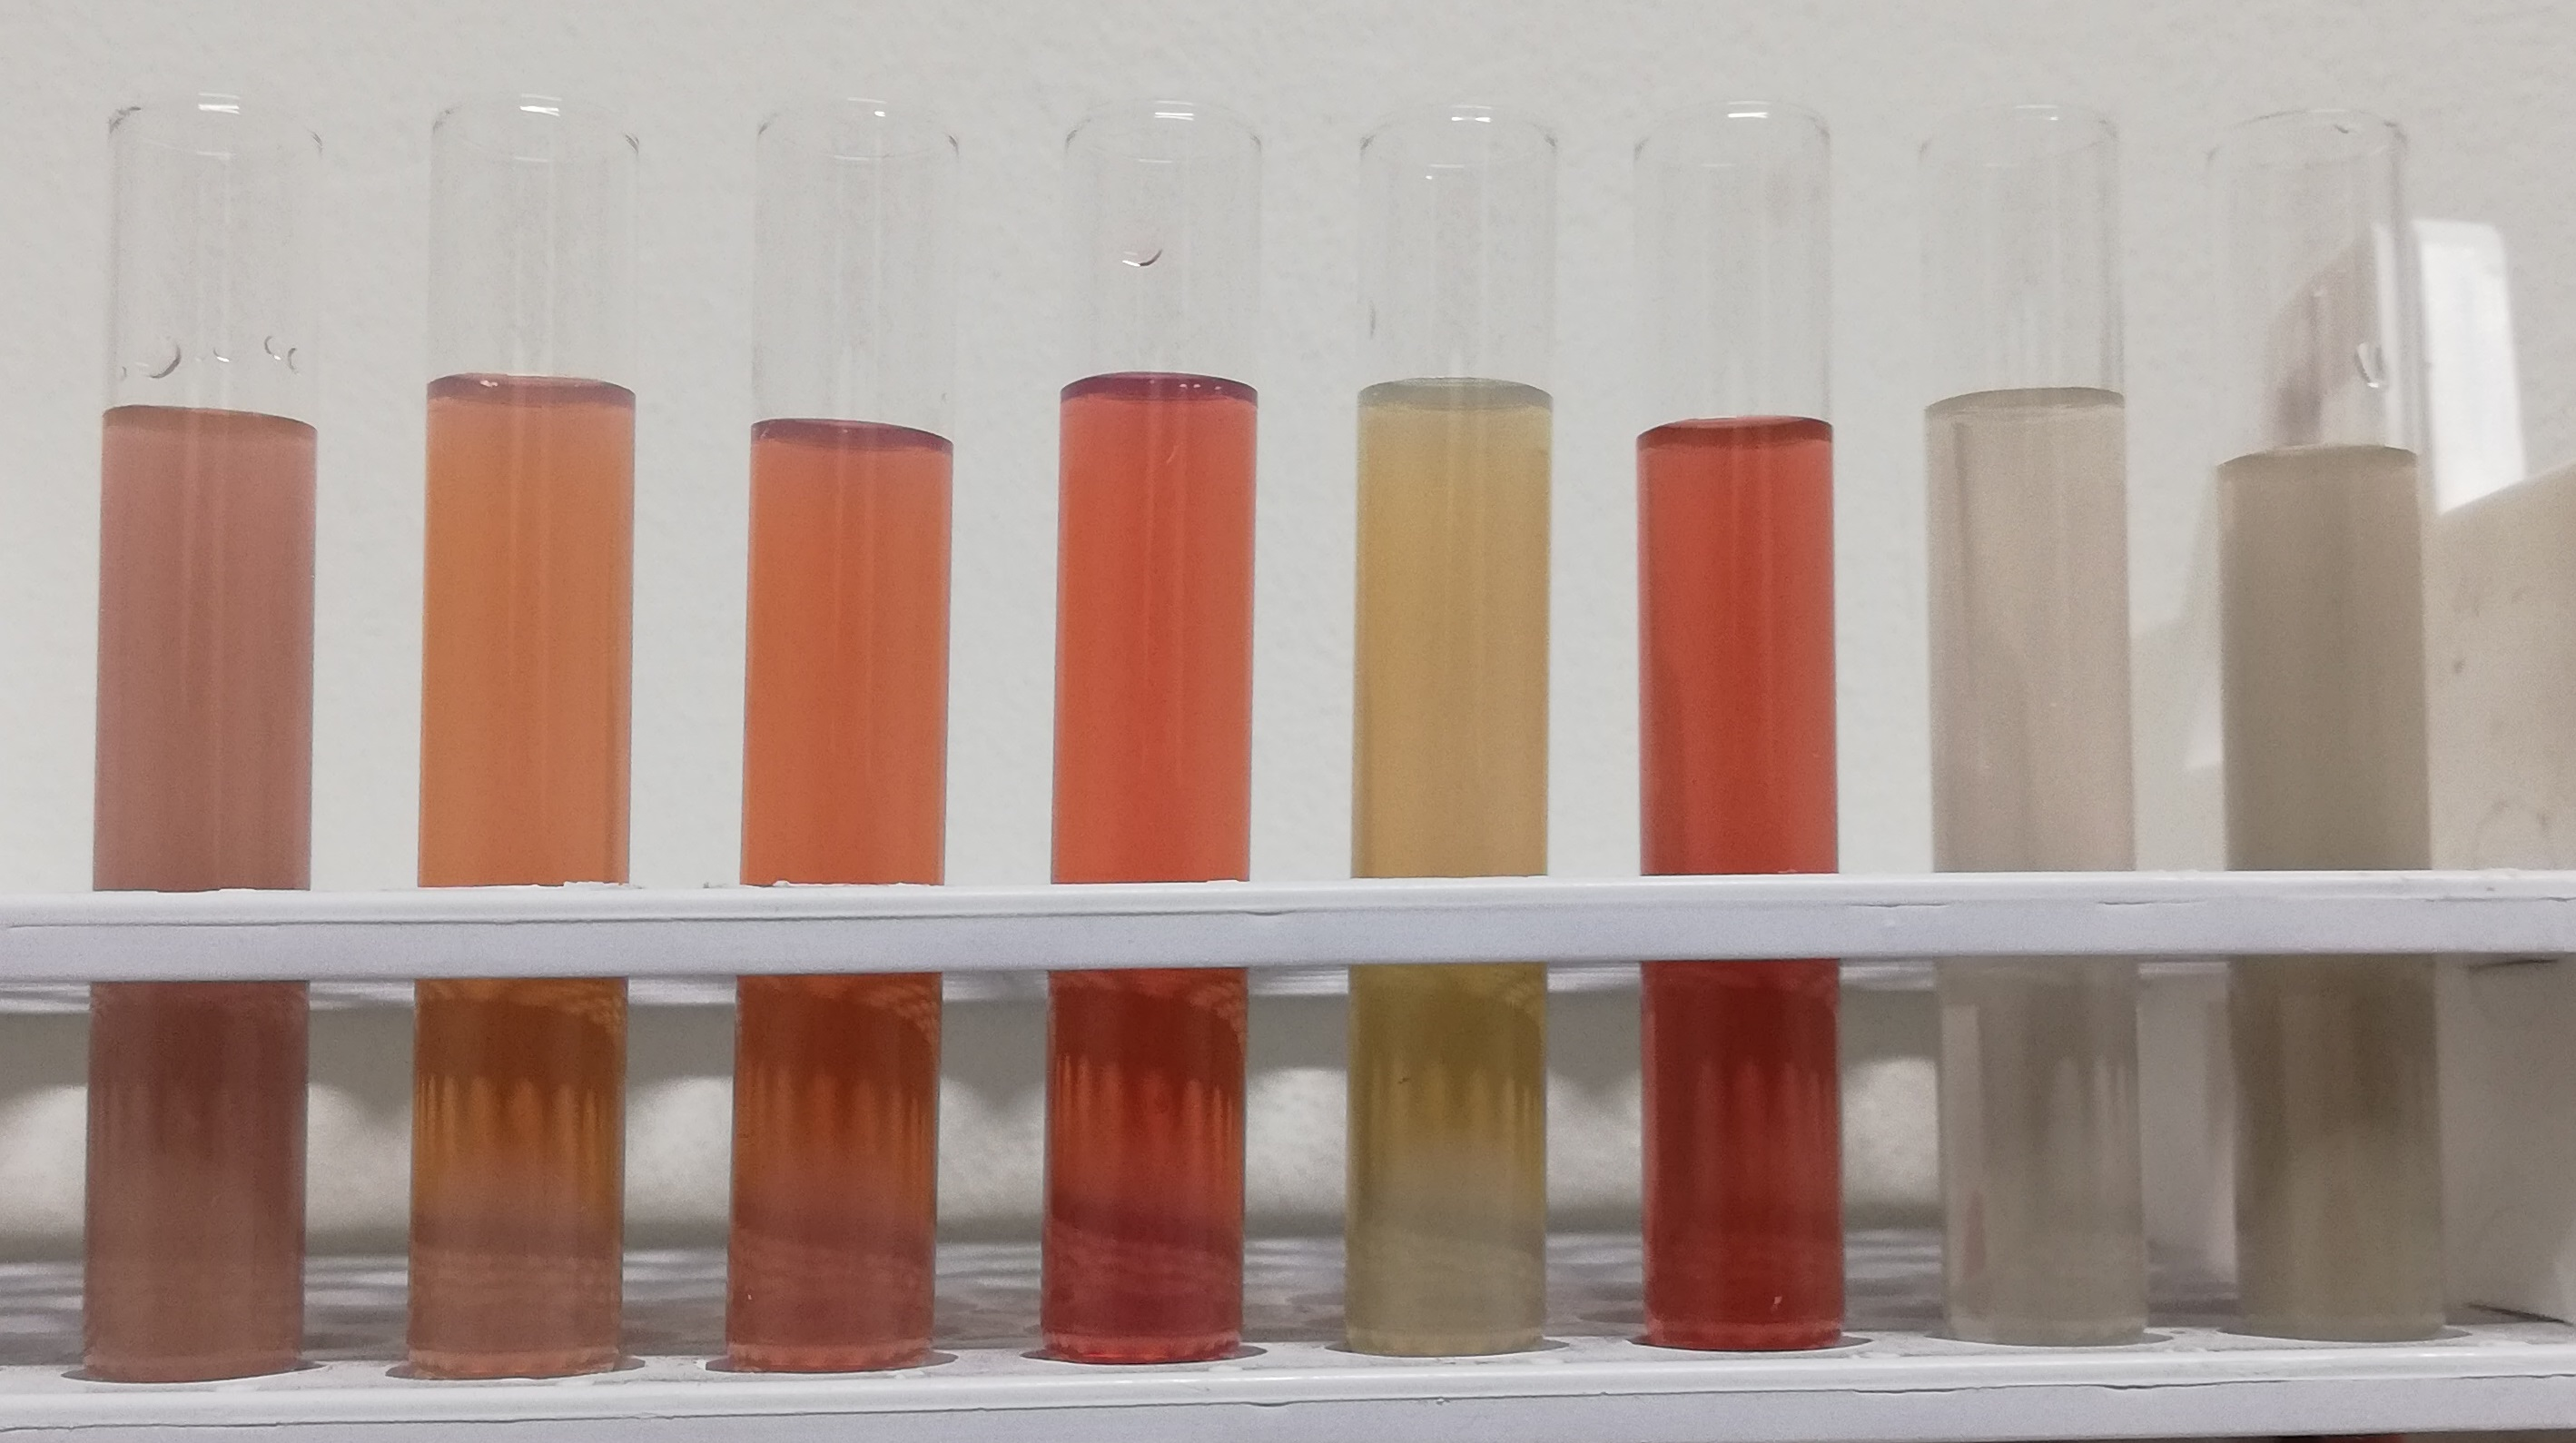
\includegraphics[width=.5\linewidth]{coverNPs}\\




\begin{textblock*}{15cm}(.25cm,8.05cm) 
\begin{flushleft} \scriptsize
Jonathan Urrutia$^1$, Corinne Luna $^2$, Gabriela Calvillo$^2$, Eugenio Méndez$^2$\\ $^1$Facultad de Ciencias, UNAM \\ $^2$Dpto. de Física Aplicada, CICESE
\end{flushleft}
\end{textblock*}

\end{frame}

%---------------------------- Title page with the diagram -------------

%---------------------------- Mie Plasmónica -------------
\section{Introducción}
\begin{frame}
\frametitle{\color{ultramarine} Plasmónica y Solución de Mie\\
\vspace*{-.25cm} \rule{\textwidth}{.5pt}   }

Solución de Mie\footfullcite{bohren}: Campo electromagnético total de una onda plana al interactuar con una partícula esférica	
	\begin{columns}
	\column{.5\textwidth} \centering

	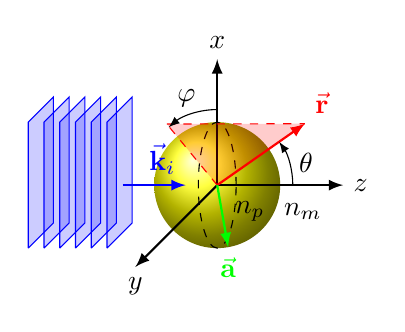
\begin{tikzpicture}[scale=.8]

\coordinate (O) at (0,0);

%------------------------------------------------------- Particle
\shade[ball color=yellow, opacity = 1] (O) circle (1); 
\draw[dashed] (O) ellipse (.3 and 1);

%------------------------------------------------------- Coordinate system axes
\draw[- latex, thick] (O) -- (-1.3,-1.3) node[anchor=north ]{$y$};
\draw[- latex, thick] (O) -- (2,0) node[anchor= west]{$z$};
\draw[- latex, thick] (O) -- (0,2) node[anchor=south]{$x$};


%------------------------------------------------------- Vector \va{r}
\draw[thick,red,- latex] (O) -- (35:1.7) node[anchor=south west]{$\va{r}$}; 
\draw[-, dashed,red] (O) -- (-.8,.97);		%xy proyection
\draw[-,dashed,red] (-.8,.97) -- (35:1.7) ;	%normal proyection
\fill[red,opacity=.2] (O)-- (-.8,.97)--(35:1.7)--(O);  %Shade
	
	
%------------------------------------------------------- polar variables	
\path (O)++(35/2:1.2)node[anchor=west]{$\theta$};    
\draw[- latex](0:1.2)arc(0:35:1.2);

\path (O)++(100:1.1)node[anchor=south east]{$\varphi$};    
\draw[- latex](90:1.2)arc(90:130:1.2);
	

%------------------------------------------------------- Particule radius & n	
\draw[thick,green,- latex] (O) -- (-80:1) node[anchor=north]{$\va{a}$};  

\path (O)++(-25:1) node[anchor=east]{$n_p$};
\path (O)++(-25:1) node[anchor=west]{$n_m$};


%------------------------------------------------------- Plane wave

\def\dx{1.75}
\def\dy{1}
\def\dr{.4}

\foreach \i in {-5,...,-1,0}{
	\fill[opacity=.2,blue] (\i*.25-\dx,-\dy)--(\i*.25-\dx,\dy)--
							(\i*.25-\dx+\dr, \dy+\dr)--(\i*.25-\dx+\dr, -\dy+\dr);
	\draw[blue] (\i*.25-\dx,-\dy)--(\i*.25-\dx,\dy)--
							(\i*.25-\dx+\dr, \dy+\dr)--(\i*.25-\dx+\dr, -\dy+\dr)--
							(\i*.25-\dx,-\dy);}									

\draw[- latex,thick,blue] (-1.5,0)--(-1.5+1,0) node[anchor=south east]{$\va{k}_i$};

	
\end{tikzpicture}

	\column{.5\textwidth}
	\begin{itemize}
		\item Partícula aislada
		\item $ \va{E}_{out} = \va{E}_{i}+\va{E}_{sca}$
		\item $\lambda$  arbitraria
		\item Radio arbitrario
	\end{itemize}		
\end{columns}
El espectro de absorción puede ser calculado.
\end{frame}

%---------------------------- Secciones transversales ------------

\begin{frame}
\frametitle{\color{ultramarine} Extinción, esparcimiento y absorción\\
\vspace*{-.25cm} \rule{\textwidth}{.5pt}   }

	\begin{columns}
	\column{.5\textwidth} \centering
	
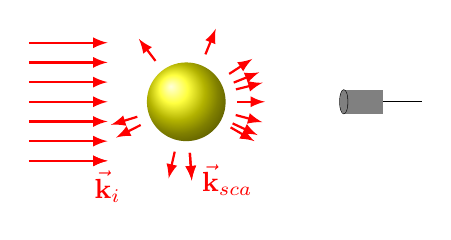
\begin{tikzpicture}[scale=.5]

\coordinate (O) at (0,0);

%------------------------------------------------------- Particle
\shade[ball color=yellow, opacity = 1] (O) circle (1); 

%------------------------------------------------------- incidence
\foreach \i in {-1.5,-1,...,1,1.5}{
	\draw[- latex,thick,red] (-4,\i)--(-2,\i);}									

\draw[- latex,thick,red] (-4,-1.5)--(-2,-1.5) node[anchor=north]{$\va{k}_i$};
%------------------------------------------------------- scat
\foreach \th in {33,68,127,274,207,197,257,-30,-25,14,22,-15,0}{
	\draw[- latex,thick,red] (\th:1.3)--(\th:2);}								

\draw[- latex,thick,red] (274:1.3)--(274:2) node[anchor=west]{$\va{k}_{sca}$};
%------------------------------------------------------- detector
\draw[black] (4,0)--(6 	,0);
\fill[gray] (4,.3)--(5,.3)--(5,-.3)--(4,-.3);
\draw[black] (4,0) ellipse (.1 and .3);
\fill[gray] (4,0) ellipse (.1 and .3);


	
\end{tikzpicture}

\begin{textblock*}{5cm}(5.1cm, 4.5cm) \centering
\begin{tikzpicture}
\shade[ball color=yellow, opacity = 1] (O) circle (.25); 
\end{tikzpicture}
\end{textblock*}

\begin{textblock*}{1cm}(1.65cm, 4.5cm) \centering
\begin{tikzpicture}
\shade[ball color=yellow, opacity = 1] (O) circle (.1); 
\end{tikzpicture}
\end{textblock*}

	\column{.5\textwidth} \centering
$$C_{ext} = C_{sca} + C_{abs}$$
$$Q = \frac{C}{\pi a^2}$$
$$Q_{ext} = Q_{sca} + Q_{abs}$$
	\end{columns}
\vspace*{-.5cm}
\begin{figure}[t!]\centering
	\begin{subfigure}{.01\linewidth}\caption{ } \vspace{2.75cm}\end{subfigure}
	\begin{subfigure}{.45\linewidth}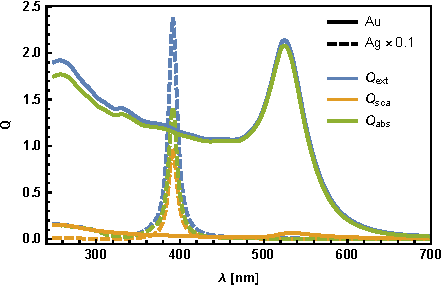
\includegraphics[width=1.0\linewidth]{TMie_r_15nm}\end{subfigure}	
	\begin{subfigure}{.01\linewidth}\caption{ }\vspace{2.75cm}	\end{subfigure}
	\begin{subfigure}{.45\linewidth}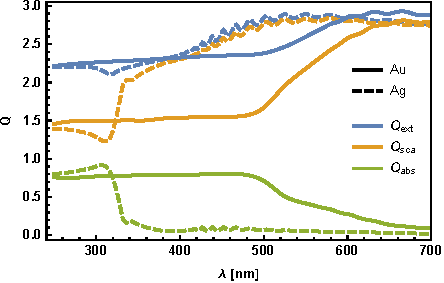
\includegraphics[width=1.0\linewidth]{TMie_r_1000nm}\end{subfigure}
	\end{figure}
\scriptsize \vspace*{-.5cm}
Eficiencia de extinción (azul), esparcimiento (naranja) y absorción (verde) para partículas de Au y Ag\footfullcite{JC1972} de \textbf{a)} 15nm y \textbf{b)} 1$\mu$m de radio inmersas en agua. 

\end{frame}


%---------------------------- Secciones transversales ------------

\begin{frame}
\frametitle{\color{ultramarine} Ley de Beer-Lambert\footfullcite{bohren}\\
\vspace*{-.25cm} \rule{\textwidth}{.5pt}   }

	\begin{columns}
	\column{.5\textwidth} \centering
	
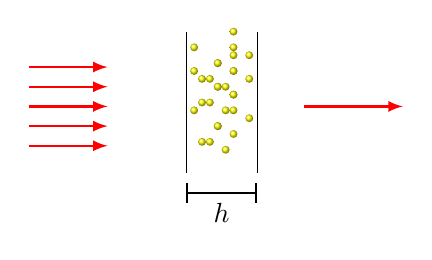
\begin{tikzpicture}[scale=.1]

\def\r{.5}
%------------------------------------------------------- Particles
	\draw[black] (0,-6)--(0,12);
	\draw[black] (9,-6)--(9,12);
\foreach \i in {0,-5,3}{
\shade[ball color=yellow, opacity = 1] (1,7+\i) circle (\r);
\shade[ball color=yellow, opacity = 1] (4,5+\i) circle (\r);
\shade[ball color=yellow, opacity = 1] (6,7+\i) circle (\r);
\shade[ball color=yellow, opacity = 1] (3,3+\i) circle (\r);
\shade[ball color=yellow, opacity = 1] (8,6+\i) circle (\r);
\shade[ball color=yellow, opacity = 1] (6,4+\i) circle (\r);
\shade[ball color=yellow, opacity = 1] (2,3+\i) circle (\r);
\shade[ball color=yellow, opacity = 1] (6,9+\i) circle (\r);
\shade[ball color=yellow, opacity = 1] (5,2+\i) circle (\r);
\shade[ball color=yellow, opacity = 1] (4,5+\i) circle (\r);}
   
   %------------------------------------------------------- incidence
\def\s{5}
\foreach \i in {-0.5,-0,...,1,1.5}{
	\draw[- latex,thick,red] (-4*\s,\s*\i)--(-2*\s,\i*\s);}							
\draw[- latex,thick,red] (3*\s,2.5)--(5.5*\s,2.5);	

\draw[|-|,thick](0,-8.5)--(9,-8.5);
\node at (4.5,-11){$h$};
	
\end{tikzpicture}

	\column{.5\textwidth} \centering
\begin{align*}
I &=  I_0 e^{-\alpha h},\\
\alpha &= \frac{N}{V} C_{ext}\\
		&=  \qty(\frac{N V_p}{V})\frac{C_{abs}+C_{sca}}{V_p}\\
		&\approx f \frac{C_{abs}}{V_p}.
\end{align*}
	\end{columns}
\vspace*{1cm}
$$f= -\frac{\ln\left( I/I_0 \right)}{C_{abs} h/V_p}$$
\end{frame}


%---------------------------- Turkevich ------------

\begin{frame}
\frametitle{\color{ultramarine} Síntesis de nanopartículas (NPs): Método de Turkevich\footfullcite{turk2015}\\
\vspace*{-.25cm} \rule{\textwidth}{.5pt}   }

\begin{textblock*}{5cm}(1.45cm, 1.45cm) \centering
1.- Reducción/Formación de cúmulos\\
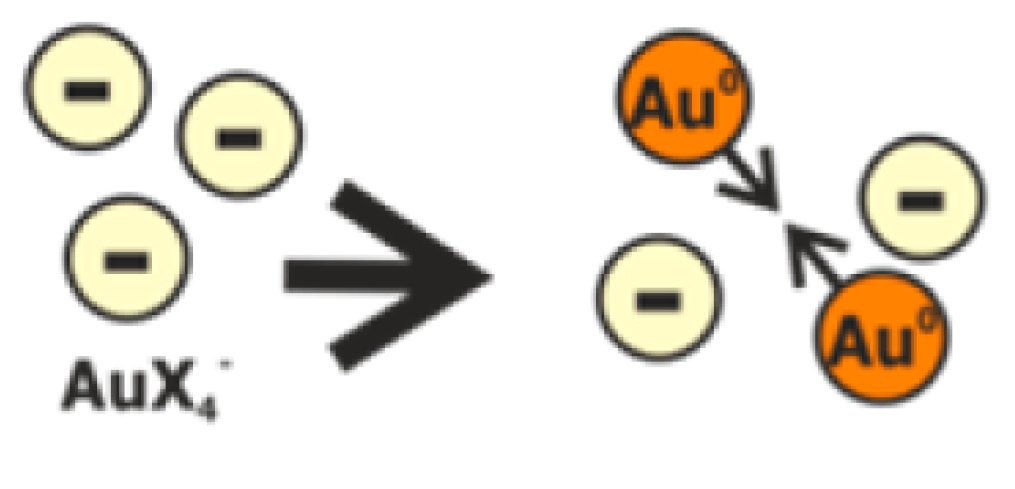
\includegraphics[scale=.2]{Turk_1}
\end{textblock*}	
\begin{textblock*}{5cm}(7cm, 1.45cm) \centering
2.- Formación de partículas \emph{semilla}\\
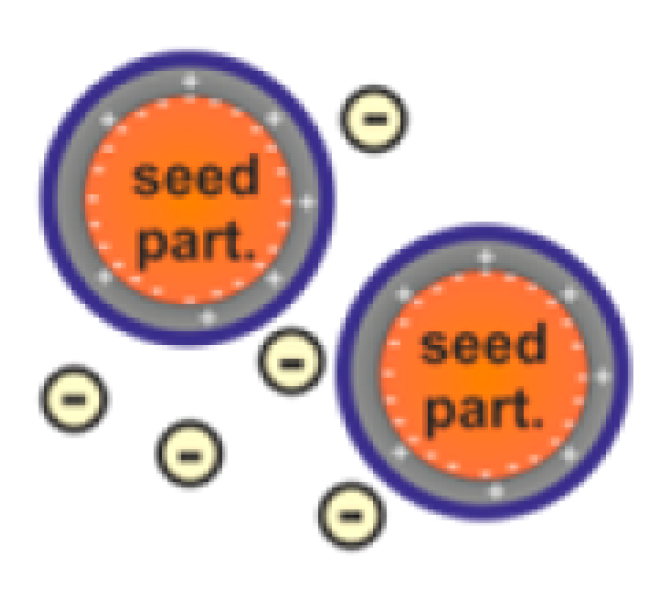
\includegraphics[scale=.2]{Turk_2}
\end{textblock*}	
\begin{textblock*}{5cm}(1.45cm, 4.5cm) \centering
3.-Crecimiento lento sobre partículas  \emph{semilla}\\
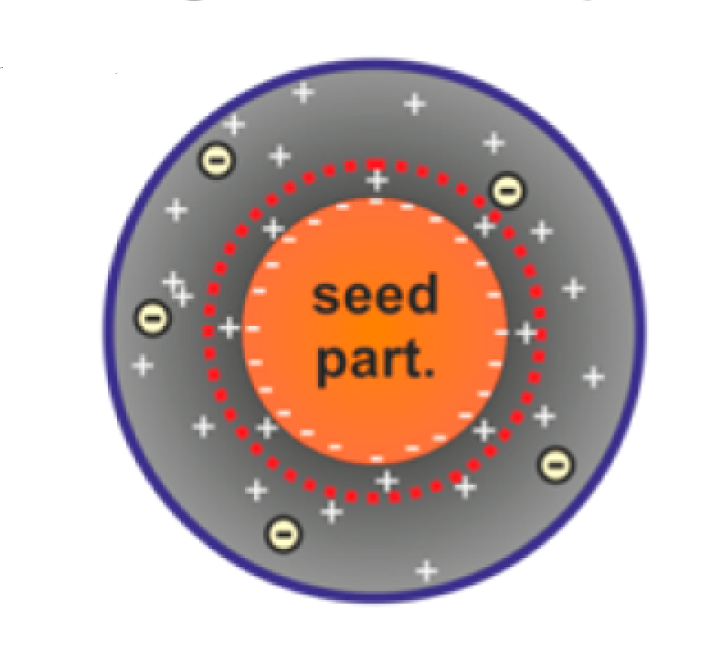
\includegraphics[scale=.2]{Turk_3}
\end{textblock*}	
\begin{textblock*}{5cm}(7cm, 4.5cm)\centering
4.-Crecimiento rápido sobre partículas  \emph{semilla}\\ 
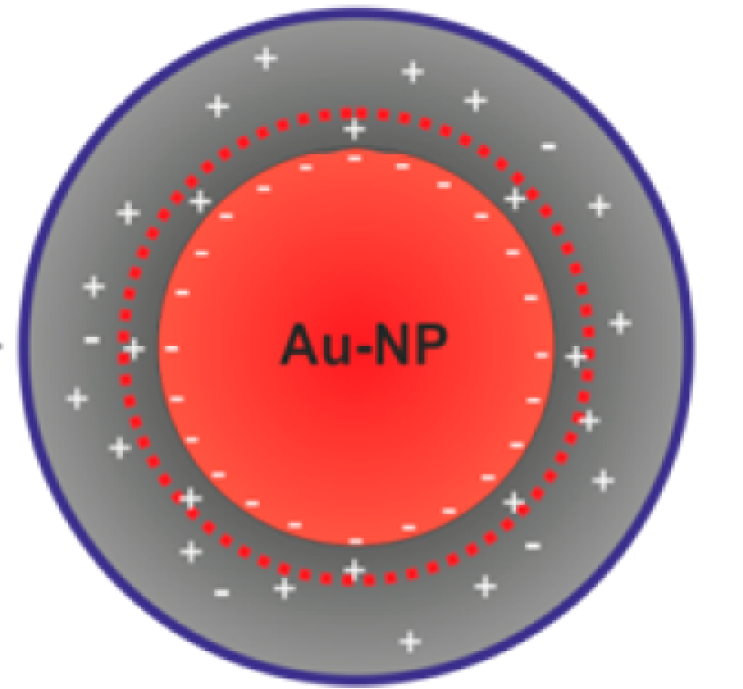
\includegraphics[scale=.2]{Turk_4}
\end{textblock*}	

\end{frame}

%---------------------------- Síntesis ------------

\begin{frame}
\frametitle{\color{ultramarine} Síntesis de NPs\\
\vspace*{-.25cm} \rule{\textwidth}{.5pt}   }\scriptsize
Proporciones para muestra coloidal de $40$ ml de NPs de Au con $2-15$nm de radio y de $90$ml de NPs de Ag con $25$nm de radio

	\begin{table}
	\begin{tabular}{c| c c c c c c}\hline \hline
	NPs & Material & $M_0$[mol/L]  & $MM$[g/mol]& $V_0$[ml] & $P_0$\\ \hline
	Au  & CIT (1\%)& $0.05000$		& $294.10$	&	$10.0$	& $0.10000$g \\	
		&HAuCl$_4$&		$0.12300$	&	$393.83$	& $2.0$	& $0.09688$g\\ \hline
	Ag & Ha		& $0.06000$		&	$33.03$		& $5.0$	& $18.38\mu$l \\
		& NaOH	&	$0.100000$	&	$40.00$		& $4.5$		& $0.01800$g\\
		& AgNO$_3$&	$0.00116$	&	$169.87$	& $90.00$		& $0.01773$g\\\hline\hline			
	\end{tabular}
	\caption{\footnotesize CIT: Citrato trisódico (Na$_3$C$_6$H$_5$O$_7$), Ha: Hidroxilamina (NH$_2$OH$\cdot$HCl) }
	\end{table}
\begin{center}
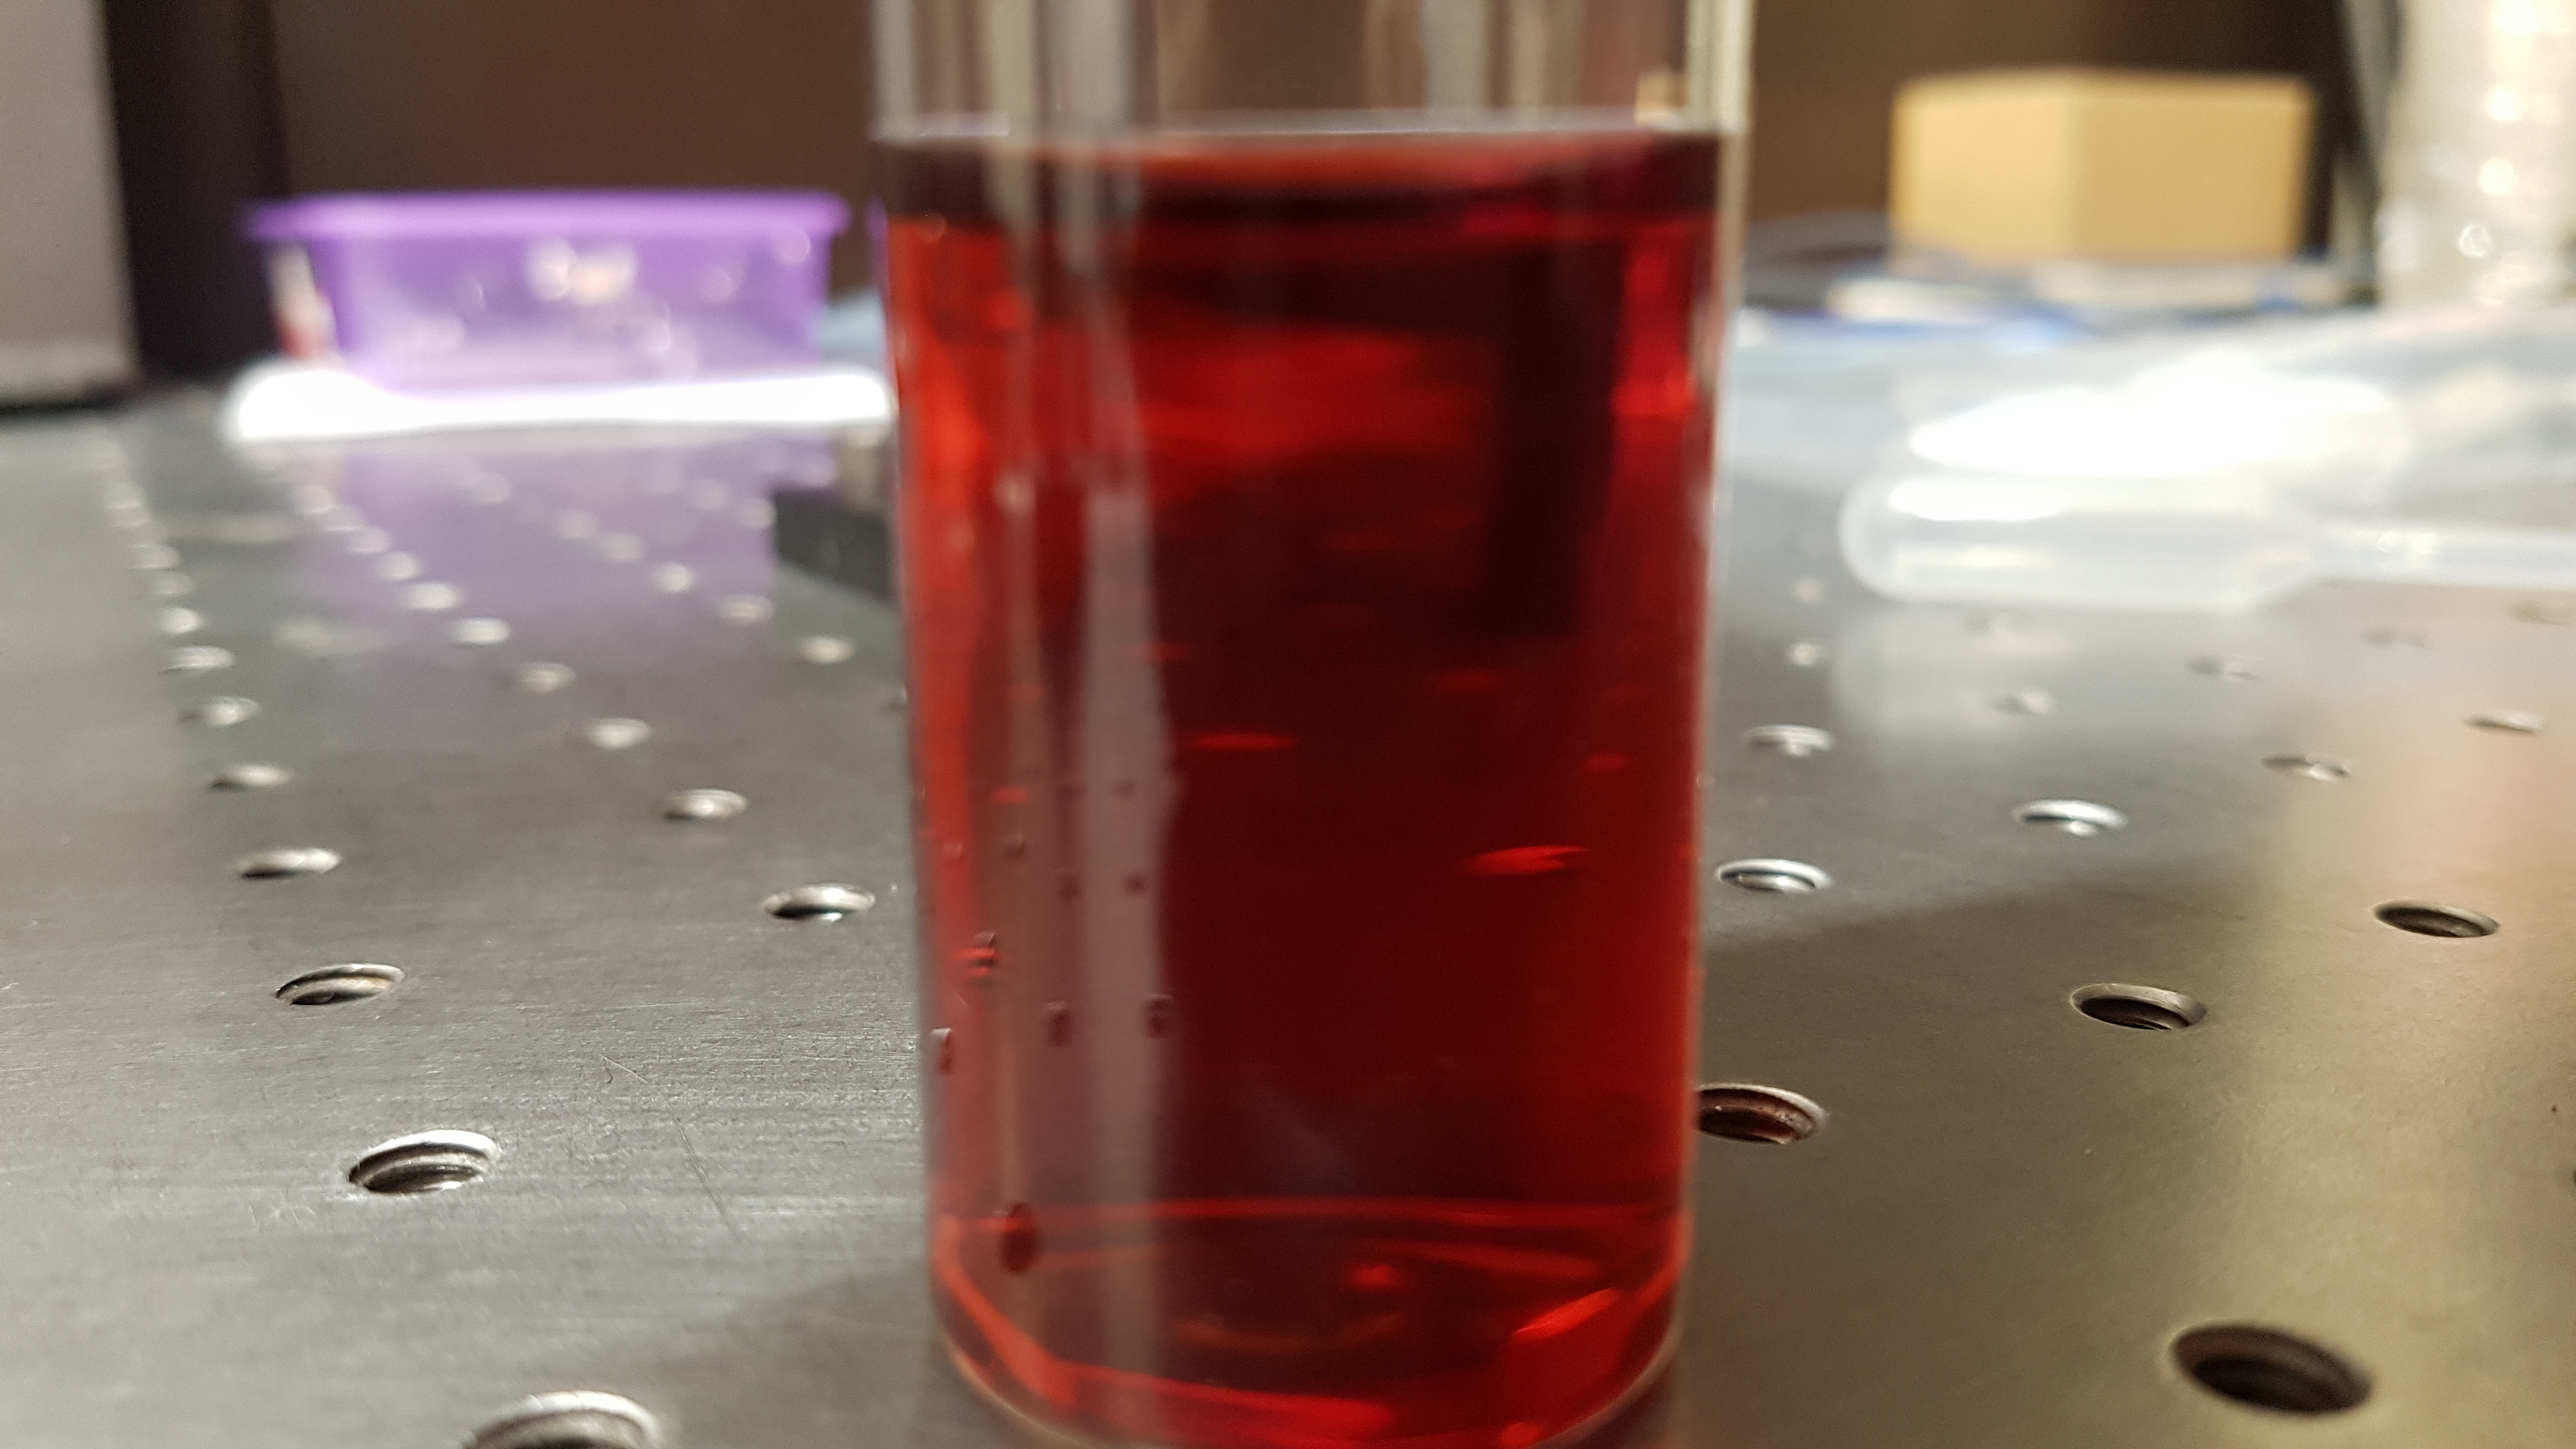
\includegraphics[width=.5\linewidth]{AuNPs}
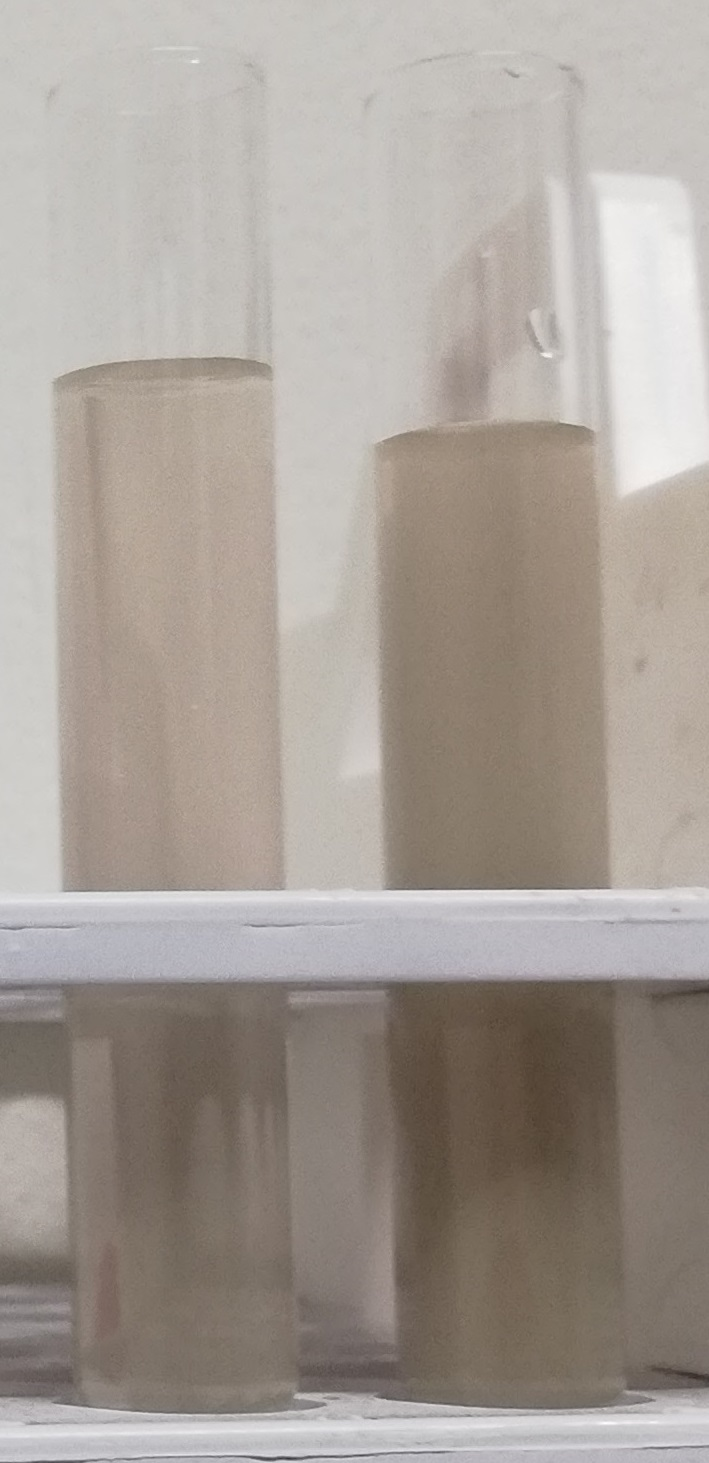
\includegraphics[scale=.06]{AgNPs}
\end{center}

\end{frame}


%---------------------------- Arreglo experimental ------------

\begin{frame}
\frametitle{\color{ultramarine} Arreglo experimental\\
\vspace*{-.25cm} \rule{\textwidth}{.5pt}   }\scriptsize
\centering
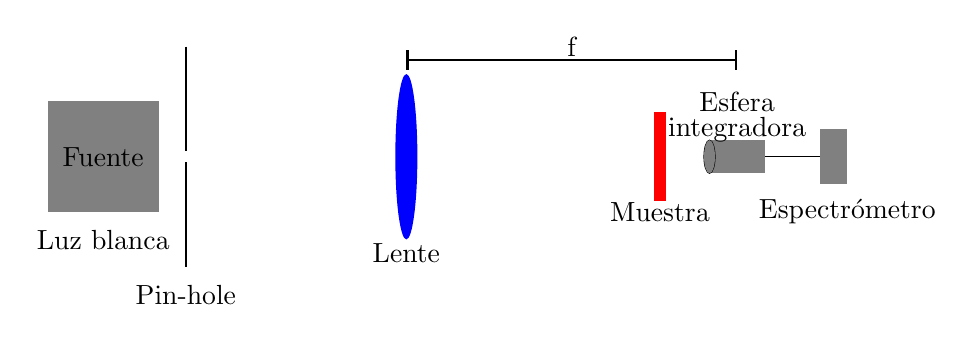
\begin{tikzpicture}[scale=.7]

\draw[fill, gray] (-1,-1)--(-1,1)--(1,1)--(1,-1)--(-1,-1);
\node at (0,0) {Fuente};
\node at (0,-1.5) {Luz blanca};

\draw[thick](1.5,2)--(1.5,.1)
			(1.5,-2)--(1.5,-.1);
\node at (1.5,-2.5) {Pin-hole};

\fill[blue] (5.5,0) ellipse (.2 and 1.5);
\node at (5.5,-1.75){Lente};

\node at (8.5,2){f};
\draw[|-|,thick] (5.5,1.75)--(11.5,1.75);			
			
\draw[fill,red](10,-.8)--(10,.8)--(10.2,.8)--(10.2,-.8);
\node at (10.1,-1){Muestra};

\def\dx{7}

\draw[black] (4+\dx,0)--(6+\dx 	,0);
\fill[gray] (4+\dx,.3)--(5+\dx,.3)--(5+\dx,-.3)--(4+\dx,-.3);

\draw[black] (4+\dx,0) ellipse (.1 and .3);
\fill[gray] (4+\dx,0) ellipse (.1 and .3);


\node at (11.5,1){Esfera};
\node at (11.5,.5){integradora};

			
\fill[gray] (13,-.5)--(13,.5)--(13.5,.5)--(13.5,-.5);	
\node at (13.5,-1){Espectrómetro}	;
\end{tikzpicture}

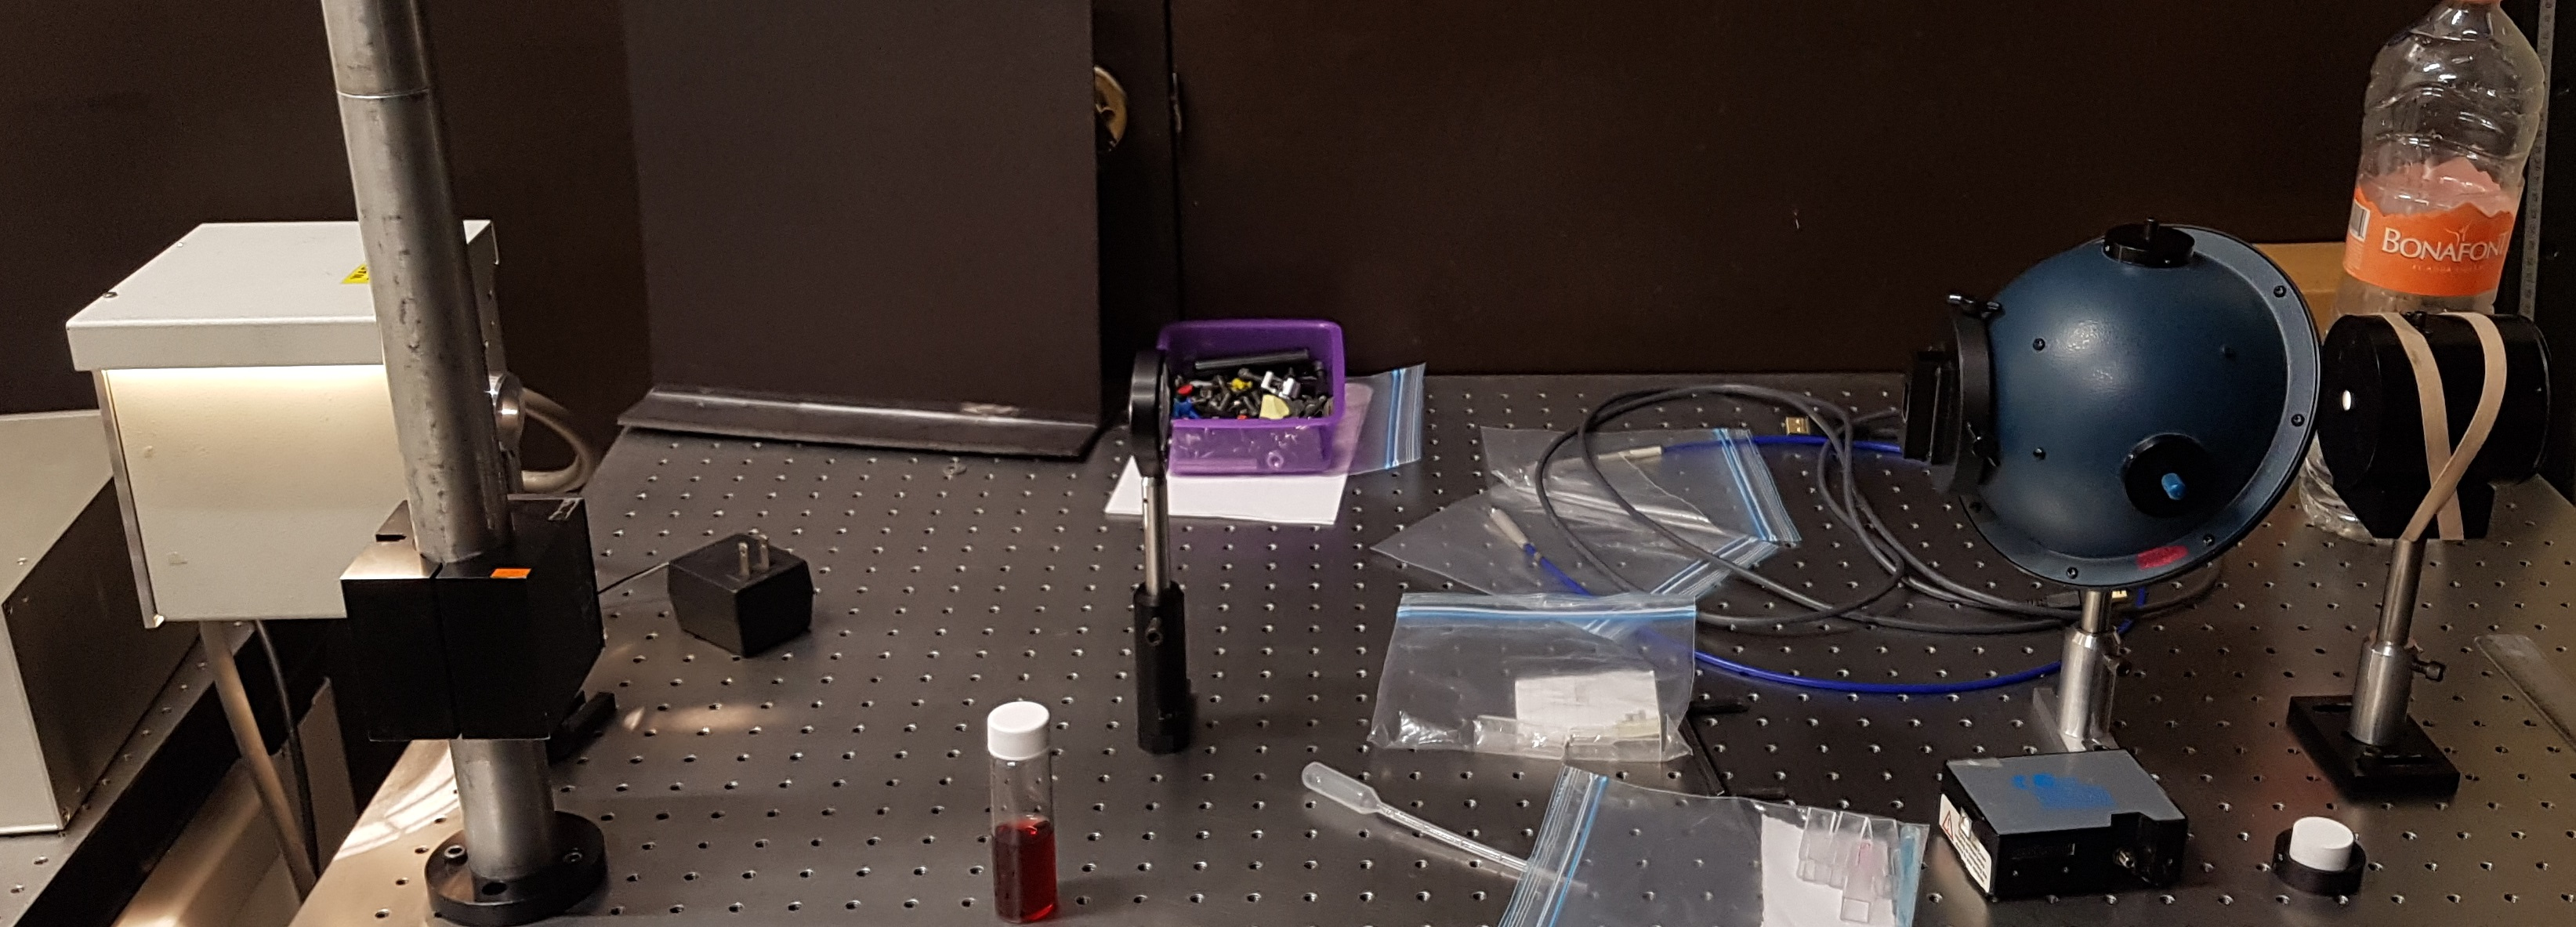
\includegraphics[width=\linewidth]{setup}

\end{frame}


%---------------------------- Absorción ------------
\begin{frame}
\frametitle{\color{ultramarine} Muestras\\
\vspace*{-.25cm} \rule{\textwidth}{.5pt}   }
\centering
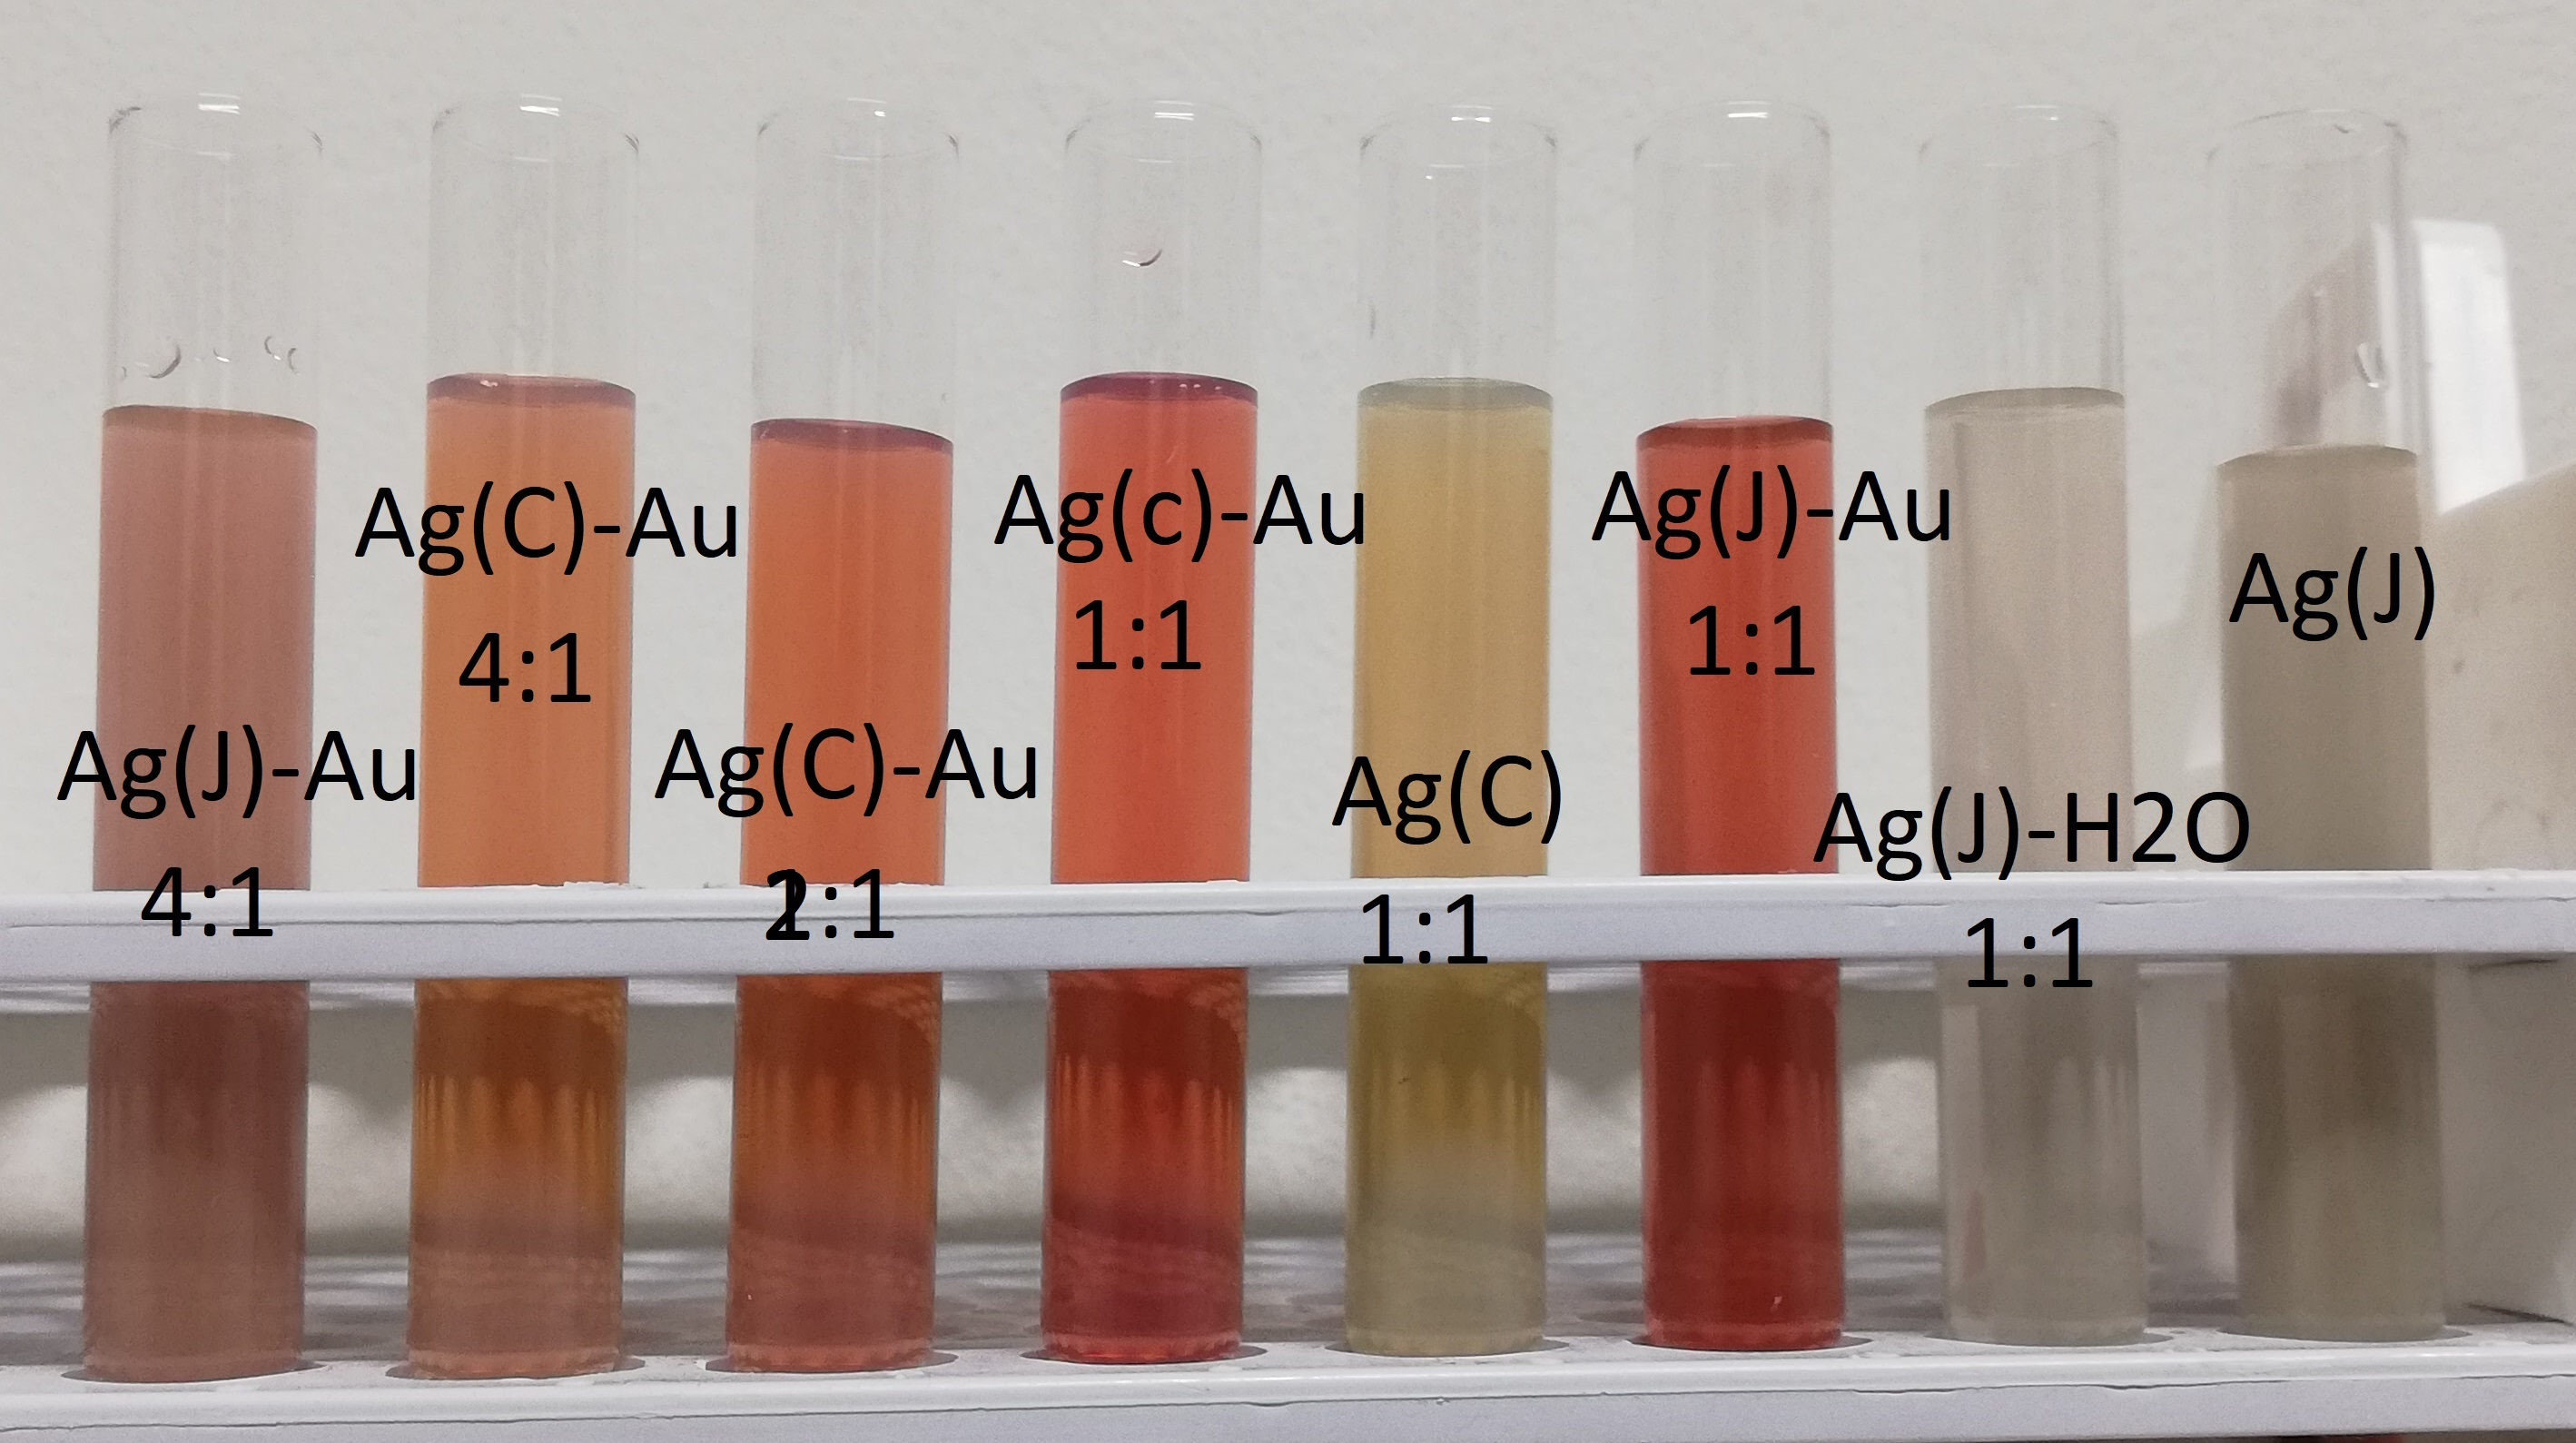
\includegraphics[width=\linewidth]{MedicionNPs}

\end{frame}


%---------------------------- Absorción ------------

\begin{frame}
\frametitle{\color{ultramarine} Espectros de absorción\\
\vspace*{-.25cm} \rule{\textwidth}{.5pt}   }
\centering
\begin{textblock*}{5cm}(6.5cm, 1.6cm)
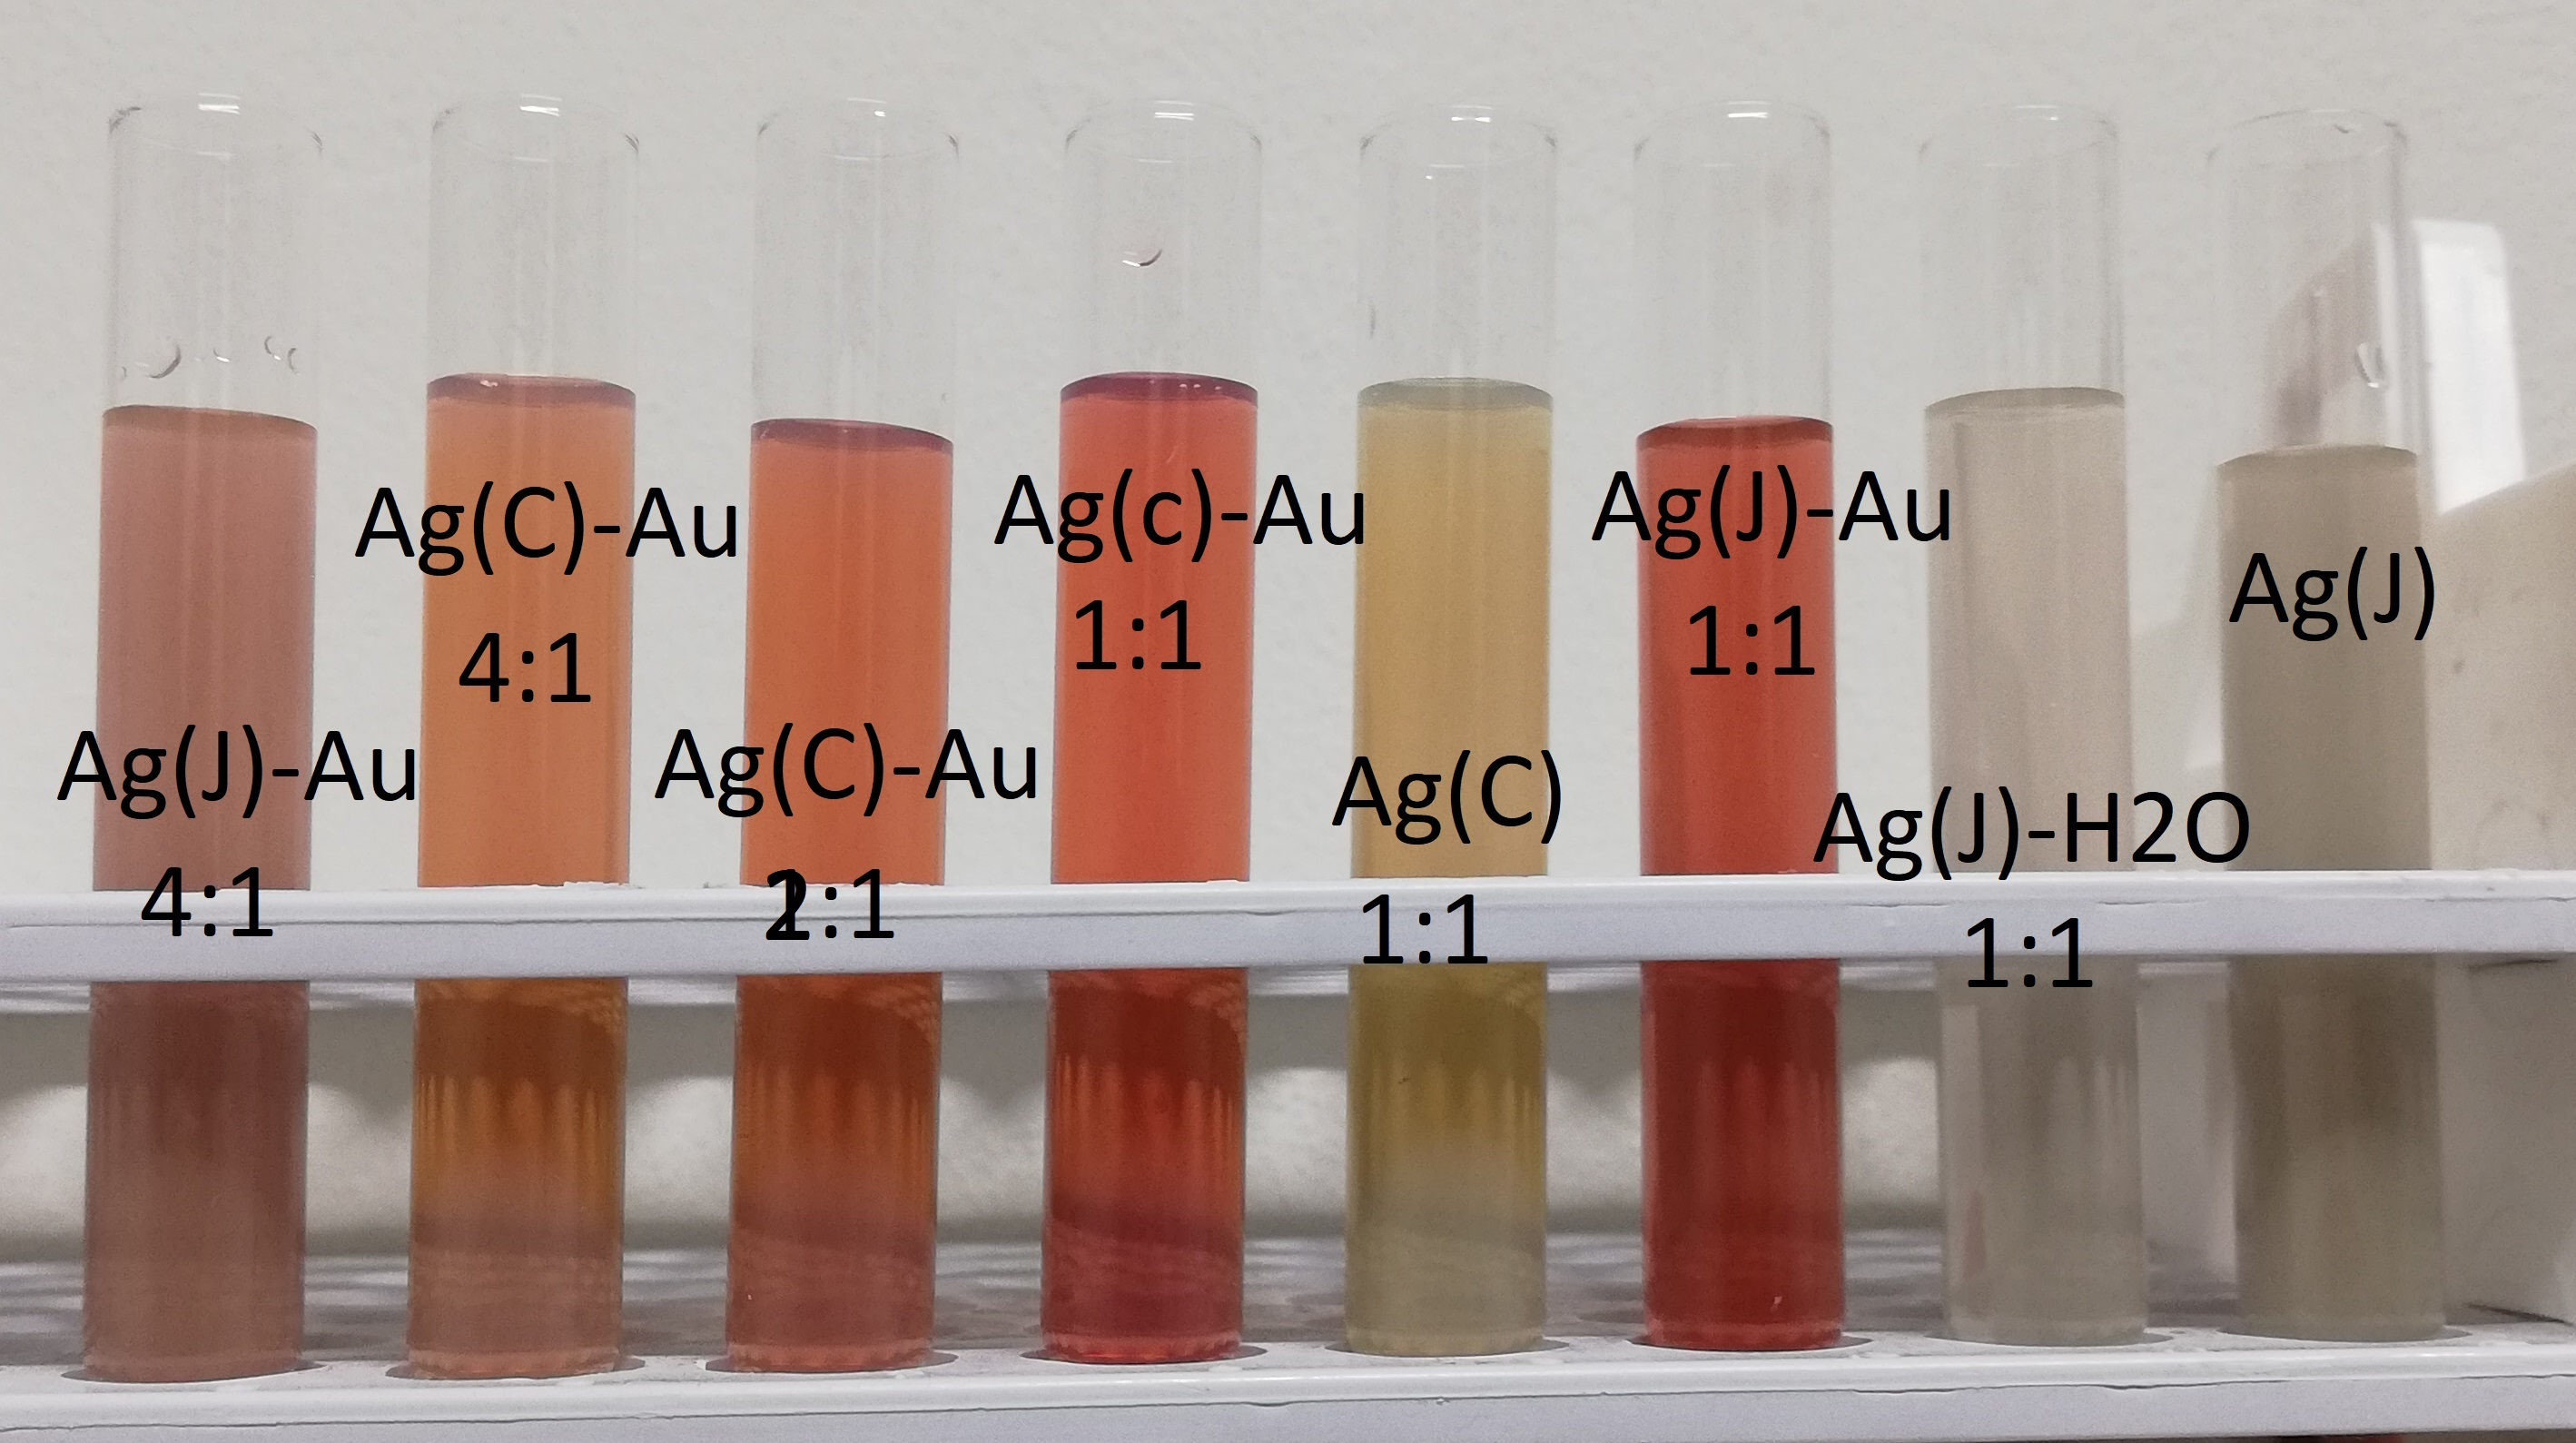
\includegraphics[scale=.06]{MedicionNPs}
\end{textblock*}	

\begin{textblock*}{5cm}(.1cm, 1.6cm)
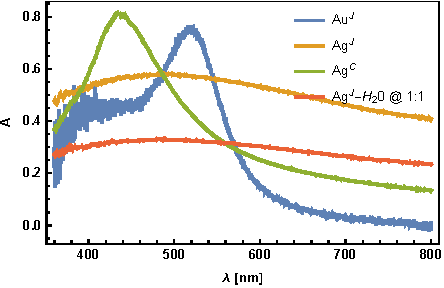
\includegraphics[scale=.85,trim={00 21 00 0}, clip]{AbsNp_1}
\end{textblock*}
\begin{textblock*}{5cm}(.1cm, 5.1cm)
\includegraphics[scale=.85]{AbsNp_2}
\end{textblock*}	
\begin{textblock*}{5cm}(6.5cm, 5.1cm)
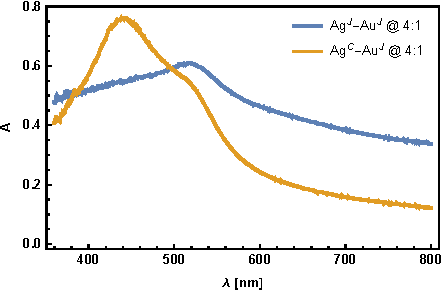
\includegraphics[scale=.85,trim={10 00 00 0}, clip]{AbsNp_3}
\end{textblock*}	


\end{frame}


%---------------------------- Absorción ------------
\begin{frame}
\frametitle{\color{ultramarine} Resultados: Au \& Ag\\
\vspace*{-.25cm} \rule{\textwidth}{.5pt}   }
\centering
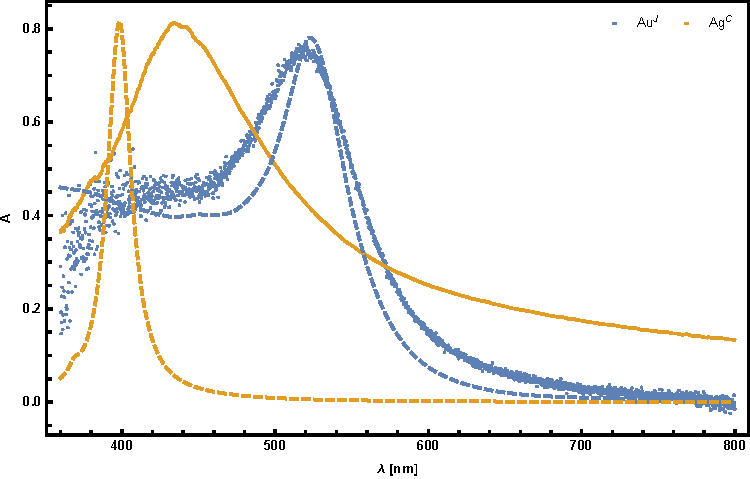
\includegraphics[width=\linewidth]{AuAg}

\begin{textblock*}{5cm}(7.25cm, 3.5cm)
$$ f_{Au}^{7.5nm} = 0.0008$$
\end{textblock*}

\begin{textblock*}{5cm}(7.25cm, 4.5cm)
$$ f_{Ag}^{20nm} = 0.00075$$
\end{textblock*}

\end{frame}


%---------------------------- Absorción ------------
\begin{frame}
\frametitle{\color{ultramarine} Muestras: Au\\
\vspace*{-.25cm} \rule{\textwidth}{.5pt}   }
\centering

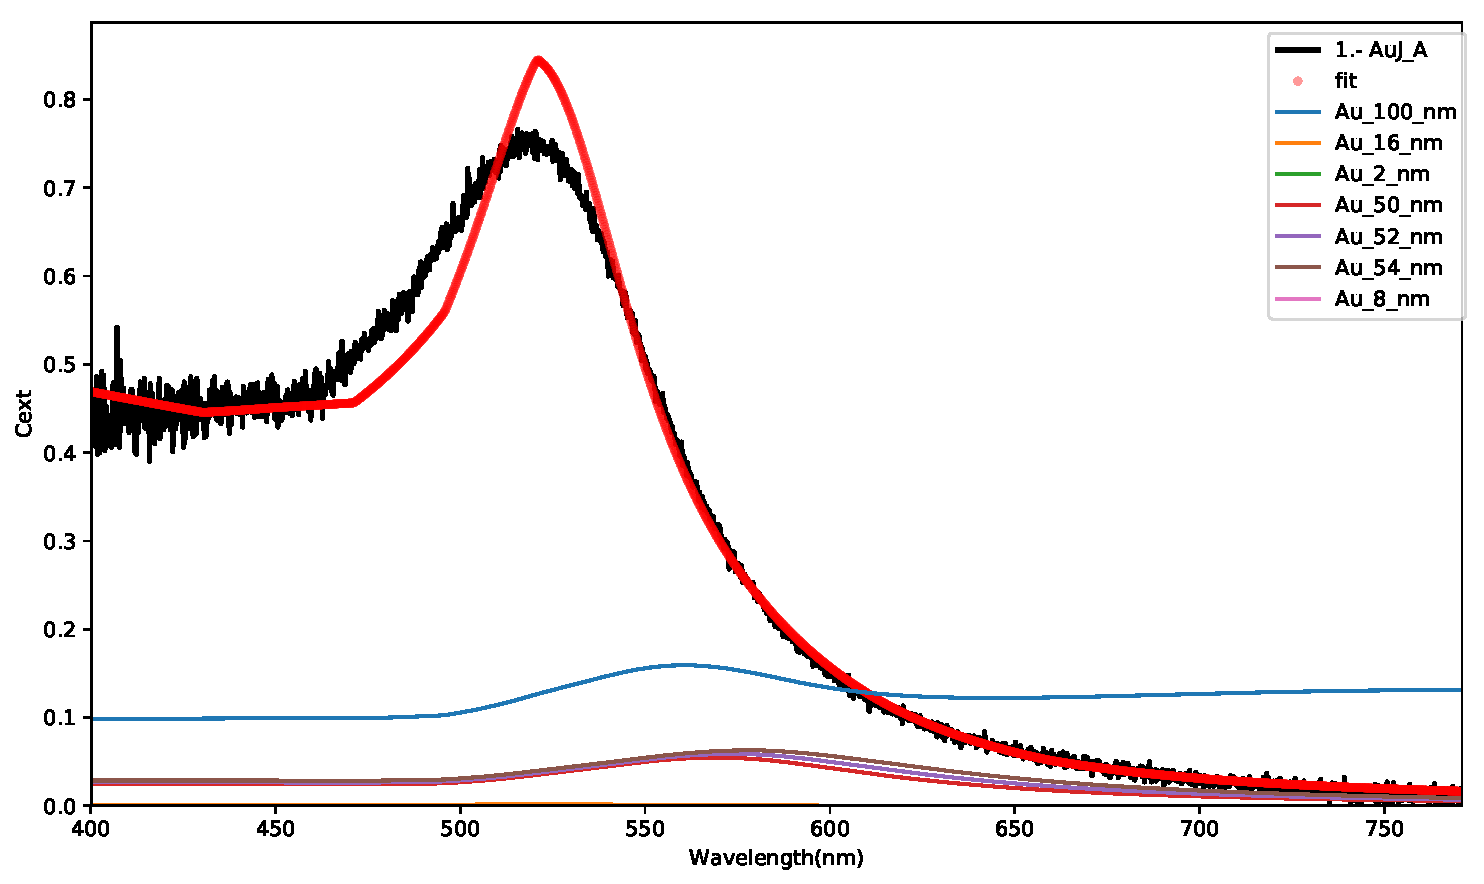
\includegraphics[width=.8\linewidth]{1-Au/fit1}

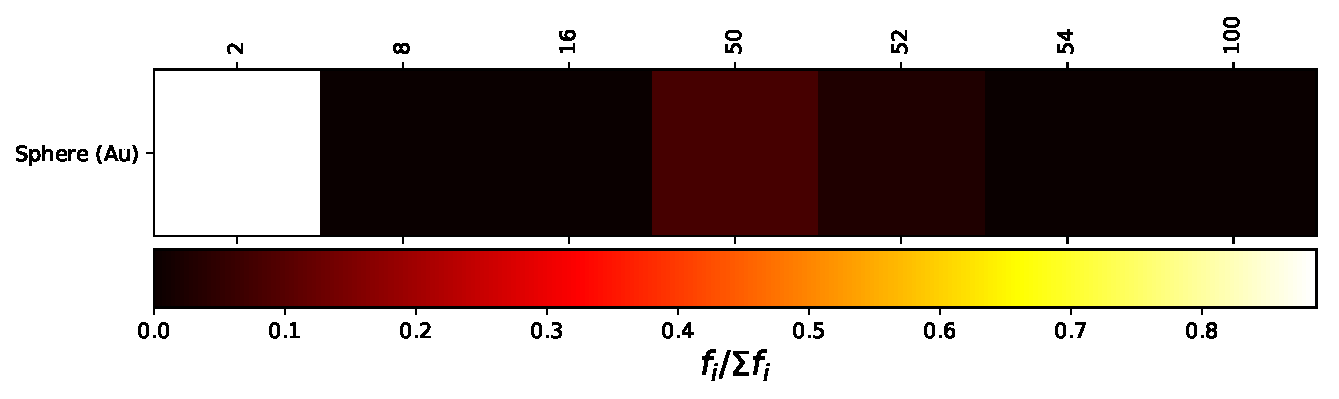
\includegraphics[width=.45\linewidth]{1-Au/fit1_volumetricfraction}
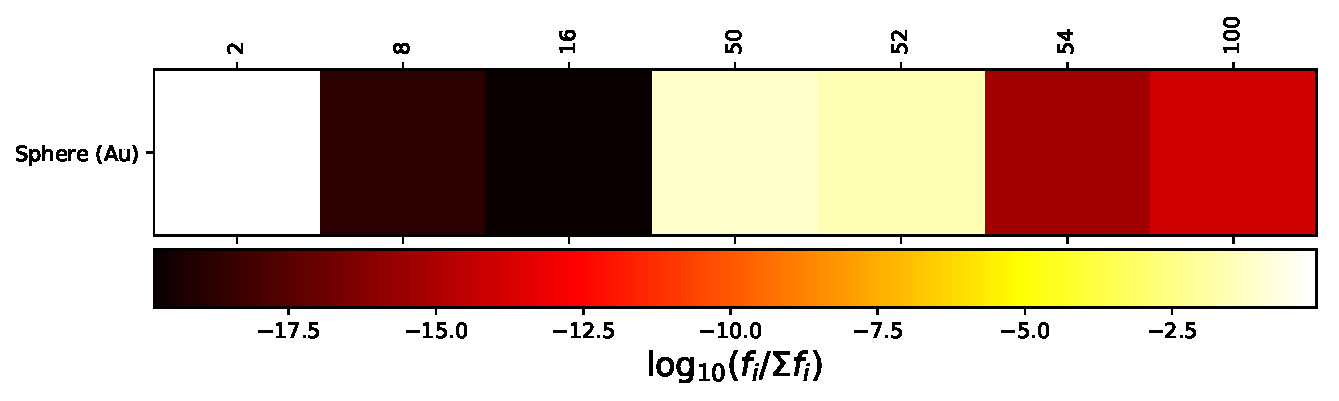
\includegraphics[width=.45\linewidth]{1-Au/fit1_volumetricfraction_logscale}
\end{frame}

\begin{frame}
\frametitle{\color{ultramarine} Muestras: Ag(C)\\
\vspace*{-.25cm} \rule{\textwidth}{.5pt}   }
\centering

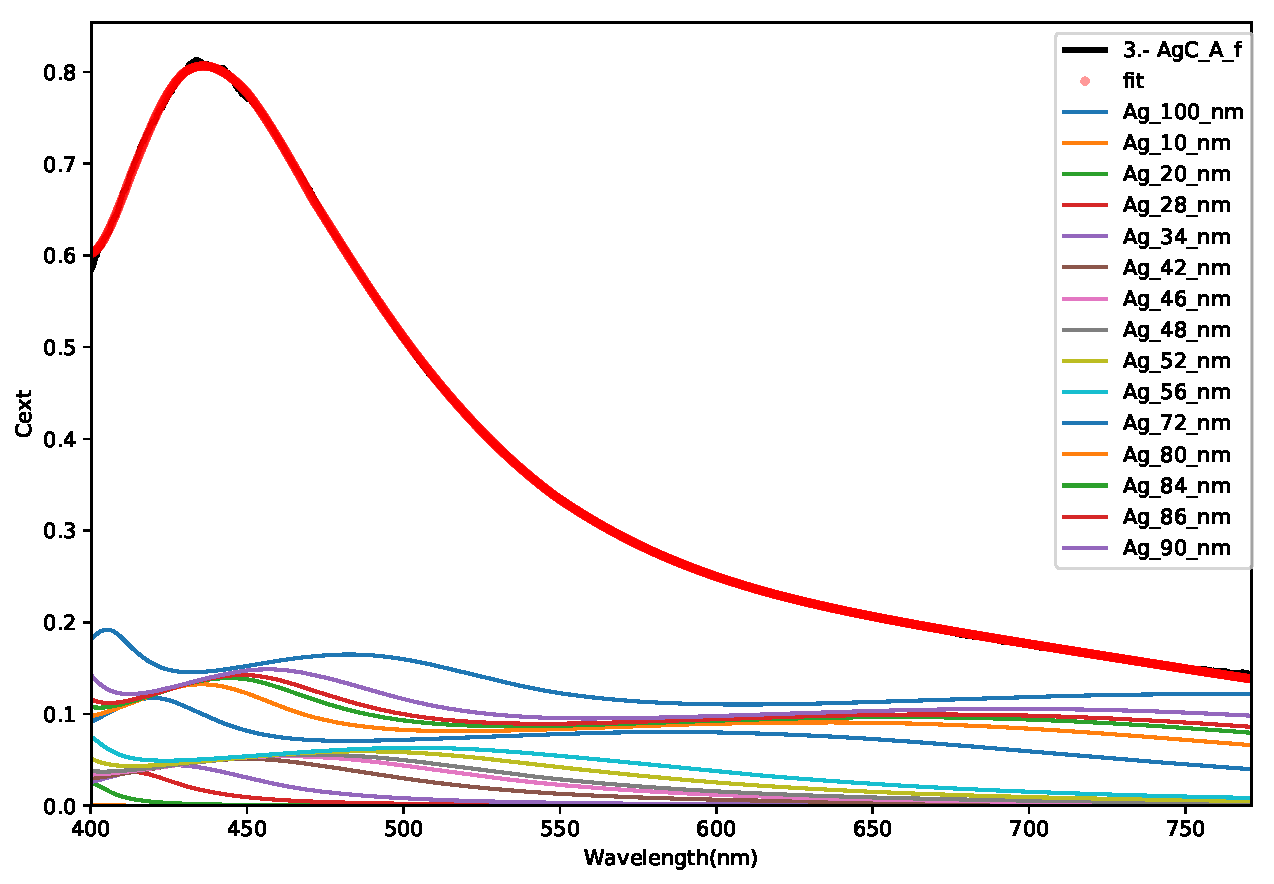
\includegraphics[width=.8\linewidth]{2-Ag/fit1}

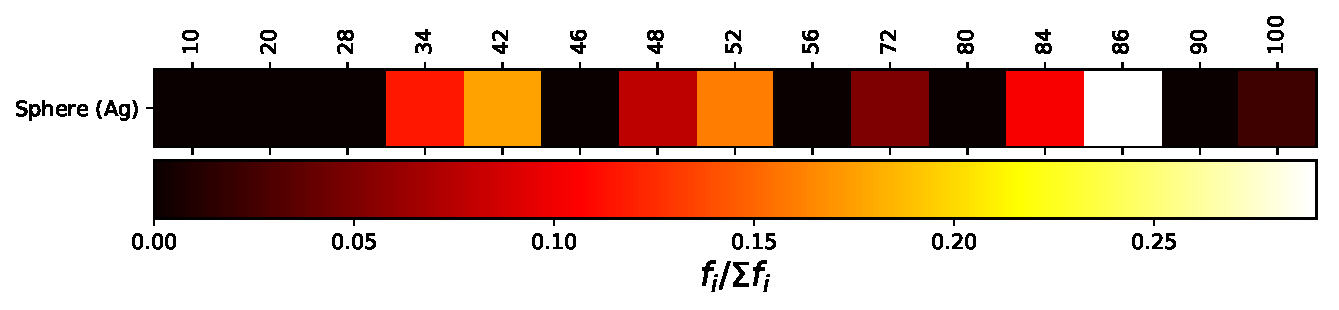
\includegraphics[width=.45\linewidth]{2-Ag/fit1_volumetricfraction}
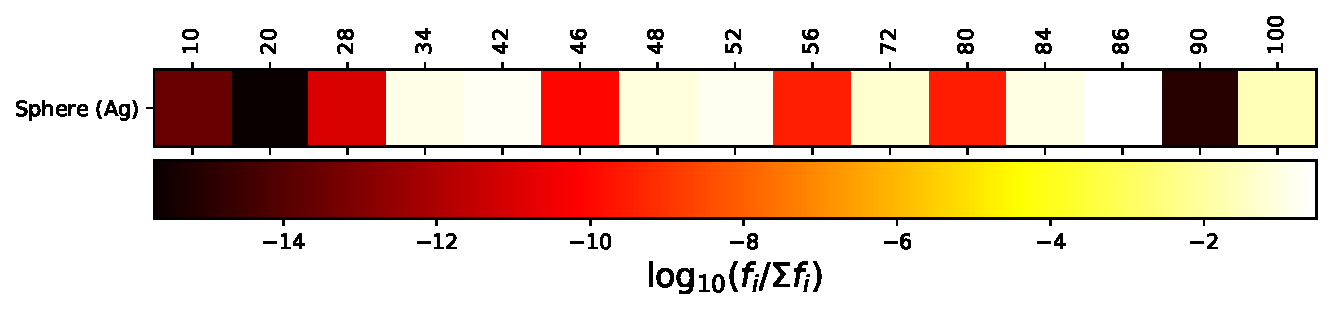
\includegraphics[width=.45\linewidth]{2-Ag/fit1_volumetricfraction_logscale}
\end{frame}


\begin{frame}
\frametitle{\color{ultramarine} Muestras: Au-Ag 1:4\\
\vspace*{-.25cm} \rule{\textwidth}{.5pt}   }
\centering

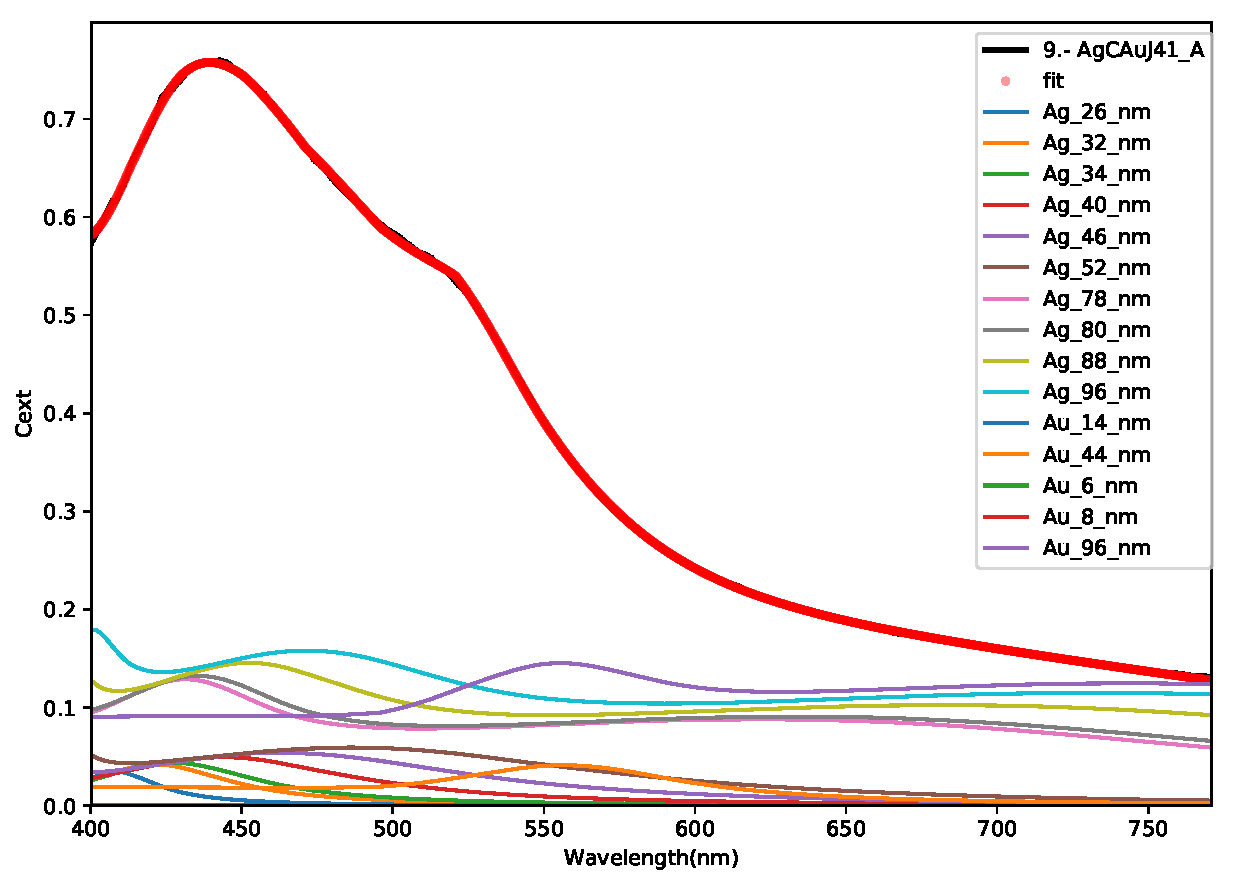
\includegraphics[width=.7\linewidth]{3-AuAg/fit1}

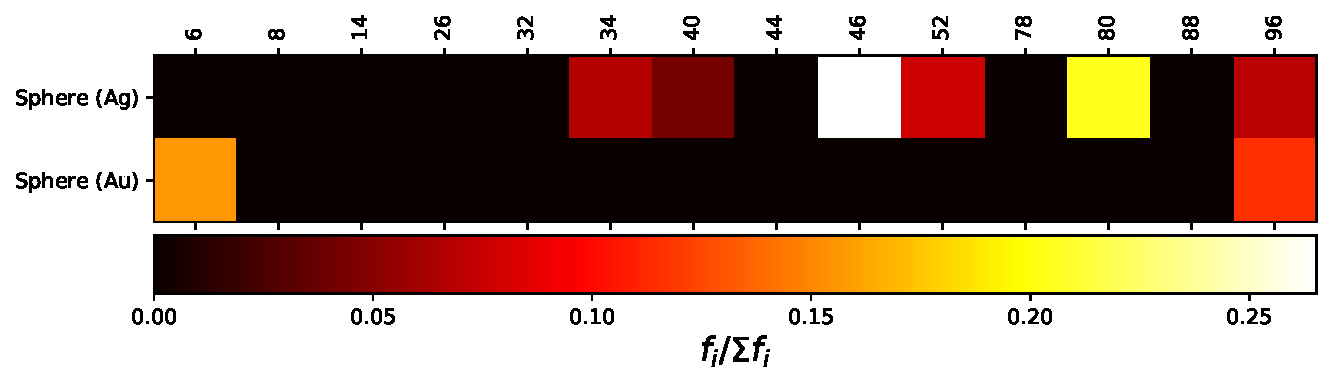
\includegraphics[width=.45\linewidth]{3-AuAg/fit1_volumetricfraction}
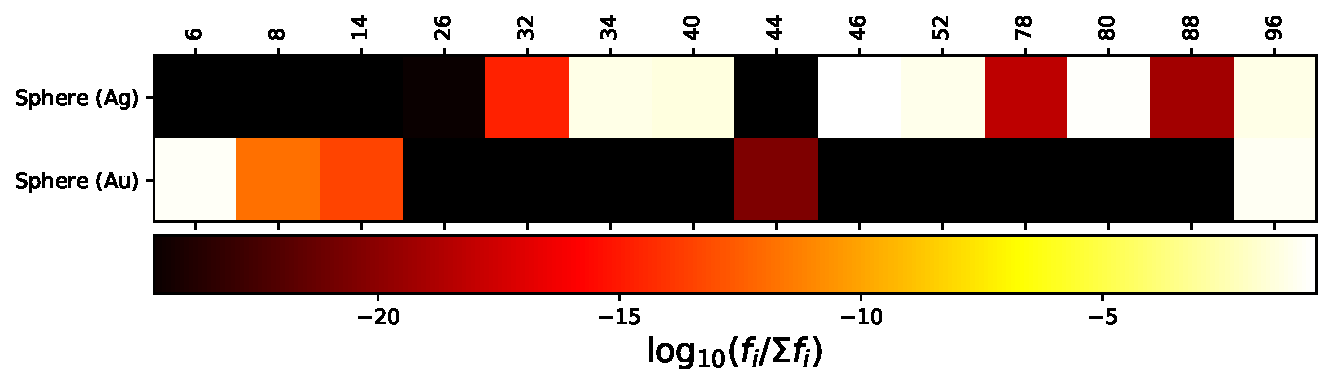
\includegraphics[width=.45\linewidth]{3-AuAg/fit1_volumetricfraction_logscale}
\end{frame}


%---------------------------- Conclusiones ------------
\begin{frame}
\frametitle{\color{ultramarine} Conclusiones\\
\vspace*{-.25cm} \rule{\textwidth}{.5pt}   }

\begin{itemize}
	\item La aproximación de $C_{ext}\approx C_{abs}$ es apropiada para simular los espectros de absorción de muestras coloidales de NPs.
	\item El espectro de extinción, la sección transversal de extinción son característicos de la geometría, tamaño, material de las NPs y medio donde se encuentran.
	\item Las características de las NPs son altamente sensibles a las condiciones y al método de síntesis.
\end{itemize}

\end{frame}










\end{document} 
